\documentclass[12pt]{article}
\usepackage[table]{xcolor}
\usepackage[shortlabels]{enumitem}
\usepackage{tabularx,xltabular}
\usepackage{graphicx}
\usepackage{hyperref}
\usepackage{verbatim}
\usepackage{geometry}
\usepackage{ulem}
\usepackage[official]{eurosym}
\usepackage{tikz}
\usetikzlibrary{arrows,backgrounds,calc,decorations.markings,patterns,3d,positioning,fit,angles, quotes}
\usepackage{pgfplots}
\pgfplotsset{compat = newest}
\usetikzlibrary{fit}
\newcommand\addvmargin[1]{
\usetikzlibrary{arrows}
\node[fit=(current bounding box),inner ysep=#1,inner xsep=0]{};}
\usepackage{cancel}
\usepackage{fontspec}
\usepackage{array}  
\geometry{a4paper, top=2cm, left=2cm, right=2cm, bottom=2cm, headsep=1cm}
\usepackage{tabu}
\usepackage{pst-node}
\usepackage{colortbl}
\usepackage{array}
\usepackage{german}
\setlength\parindent{0pt}
\newcolumntype{?}{!{\vrule width 1pt}}
\usepackage{makecell}
\renewcommand{\arraystretch}{2.5}
\usepackage{pbox}
\usepackage{amssymb}
\usepackage{amsmath}
\usepackage{booktabs}
\newcolumntype{L}[1]{>{\raggedright\let\newline\\\arraybackslash\hspace{0pt}}m{#1}}
\newcolumntype{C}[1]{>{\centering\let\newline\\\arraybackslash\hspace{0pt}}m{#1}}
\newcolumntype{R}[1]{>{\raggedleft\let\newline\\\arraybackslash\hspace{0pt}}m{#1}}
\begin{document}
\pgfmathsetmacro{\pkteAfgEins}{12}
\pgfmathsetmacro{\pkteAfgZwei}{8}
\pgfmathsetmacro{\pkteAfgDrei}{0}
\pgfmathsetmacro{\pkteAfgVier}{0}
\pgfmathsetmacro{\pkteAfgFuenf}{0}
\pgfmathsetmacro{\pkteAfgSechs}{0}
\pgfmathsetmacro{\pkteAfgSieben}{0}
\pgfmathsetmacro{\sauberkeitsPkte}{2}
\def\datum{12.12.2023}
\def\kurs{~}
\def\titel{Prozent und Zinsrechnung}
\def\jahr{2022/2023}
\def\fach{Mathematik}
\def\name{~}
\def\material{Füller / Kugelschreiber / Fineliner, Bleistift, Taschenrechner}
\pgfmathsetmacro{\gesPkte}{\pkteAfgEins+\pkteAfgZwei+\pkteAfgDrei+\pkteAfgVier+\pkteAfgFuenf+\pkteAfgSechs+\pkteAfgSieben+\sauberkeitsPkte}
%Mit den folgenden Zeilen werden die Nummern nicht angezeigt, bei denen die Aufgaben 0 Punkte haben.
\newcommand{\Eins}{~}
\newcommand{\pEins}{~}
\ifnum\pkteAfgEins>0  \renewcommand{\Eins}{1} \fi
\ifnum\pkteAfgEins>0  \renewcommand{\pEins}{\pkteAfgEins} \fi
\newcommand{\Zwei}{~}
\newcommand{\pZwei}{~}
\ifnum\pkteAfgZwei>0  \renewcommand{\Zwei}{2} \fi
\ifnum\pkteAfgZwei>0  \renewcommand{\pZwei}{\pkteAfgZwei} \fi
\newcommand{\Drei}{~}
\newcommand{\pDrei}{~}
\ifnum\pkteAfgDrei>0  \renewcommand{\Drei}{3} \fi
\ifnum\pkteAfgDrei>0  \renewcommand{\pDrei}{\pkteAfgDrei} \fi
\newcommand{\Vier}{~}
\newcommand{\pVier}{~}
\ifnum\pkteAfgVier>0  \renewcommand{\Vier}{4} \fi
\ifnum\pkteAfgVier>0  \renewcommand{\pVier}{\pkteAfgVier} \fi
\newcommand{\Fuenf}{~}
\newcommand{\pFuenf}{~}
\ifnum\pkteAfgFuenf>0  \renewcommand{\Fuenf}{5} \fi
\ifnum\pkteAfgFuenf>0  \renewcommand{\pFuenf}{\pkteAfgFuenf} \fi
\newcommand{\Sechs}{~}
\newcommand{\pSechs}{~}
\ifnum\pkteAfgSechs>0  \renewcommand{\Sechs}{6} \fi
\ifnum\pkteAfgSechs>0  \renewcommand{\pSechs}{\pkteAfgSechs} \fi
\newcommand{\Sieben}{~}
\newcommand{\pSieben}{~}
\ifnum\pkteAfgSieben>0  \renewcommand{\Sieben}{7} \fi
\ifnum\pkteAfgSieben>0  \renewcommand{\pSieben}{\pkteAfgSieben} \fi
\newcommand{\sauber}{~}
\newcommand{\pSauber}{~}
\ifnum\sauberkeitsPkte>0  \renewcommand{\sauber}{SK} \fi
\ifnum\sauberkeitsPkte>0  \renewcommand{\pSauber}{\sauberkeitsPkte} \fi
\pagenumbering{gobble}
\begin{tabularx}{\textwidth}{ R{2.0cm} X R{2.0cm}  }
&
{\centering{\Large\bf
\fach\\
\titel}\\ 
Schuljahr \jahr\par
} &
\end{tabularx} \\
\begin{tabularx}{\textwidth}{R{2.0cm} X R{2.0cm} X }
Name: & \name& Kurs:  & \kurs\\\cline{2-2}\cline{4-4}
& & Datum:& \datum \\\cline{2-2}\cline{4-4}
\end{tabularx} \\
\phantom{M}\\
{\bf\underline{Benötigtes Material}}\\
\vspace{-0.5cm}
\begin{itemize}
\itemsep0em 
\foreach \x in \material
{\item \x }
\end{itemize}

{\bf\underline{Ablauf:}}\\
Nach dem Verteilen der Arbeit schreibst du auf jedem Zettel deinen Namen. Lege danach dein Stift wieder weg. Wenn alle die Arbeit haben, fangen wir an. Du hast 45 min Zeit zur Bearbeitung der Aufgaben.
\\
{\bf\underline{Allgemeines:}}\\
\vspace{-0.5cm}
\begin{enumerate}
\itemsep0em 
\item Während der Arbeit darf nicht miteinander gesprochen werden. Willst Du was sagen, melde dich.
\item Wenn Dir eine Aufgabenstellung unklar ist, melde Dich.
\item Wer schummelt hat verloren!
\end{enumerate}

\begin{tabularx}{\textwidth}{|X|C{1cm}|C{1cm}|C{1cm}|C{1cm}|C{1cm}|C{1cm}|C{1cm}|C{1cm}|C{1cm}|}
\hline
Aufgabe & \Eins&\Zwei&\Drei&\Vier&\Fuenf&\Sechs&\Sieben& \sauber & $\sum$ \\\hline
Mögliche Punkte &\pEins&\pZwei&\pDrei&\pVier&\pFuenf&\pSechs&\pSieben&  \pSauber&\pgfmathprintnumber{\gesPkte} \\\hline
Erreichte Punkte& & & & & & & &  & \\\hline
\end{tabularx}\\
\phantom{M} \\
\begin{tabularx}{\textwidth}{|c| }
\hline 
{\bf Erreichte Note}\\\hline
\parbox[c][3cm]{16.55cm}{\phantom{M}} \\\hline
\end{tabularx} 
{\centering{\large\bf
Gleich geht’s los! Viel Erfolg!
\par
}}
\newpage
\pagenumbering{arabic}
\pgfmathsetmacro{\punkte}{\pkteAfgEins}
\newpage
\section{Prozent- und Zinsrechnung}
\subsection{Erkennen den Prozentwert}
Füge hier bitte einen Beschreibungstext ein. Behalte die beiden Backslash \textbackslash\textbackslash. Die bedeuten eine neue Zeile. Soll die Aufgabe nicht auf einer neuen Seite beginnen, entferne den Befehl \textbackslash newpage am Anfang der tex-Datei.\\
\begin{xltabular}{\textwidth}{|C{0.75cm}|X|}
\arrayrulecolor{black}\hline
a)&\tikzstyle{background grid}=[draw, black!15,step=.5cm]
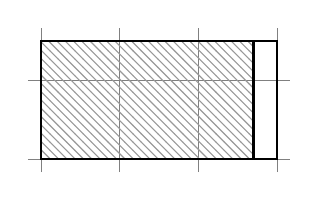
\begin{tikzpicture}[show background grid]
\pgfmathsetmacro{\laenge}{3}  
\pgfmathsetmacro{\hoehe}{\laenge/2}  
\pgfmathsetmacro{\percent}{90/100}  
\draw[thick] (0,0) rectangle ++ (\laenge,\hoehe);
\draw[thick,pattern=north west lines, pattern color=black!40] (0,0) rectangle ++ (\laenge*\percent,\hoehe);
\end{tikzpicture}
\\\hline
b)&\tikzstyle{background grid}=[draw, black!15,step=.5cm]
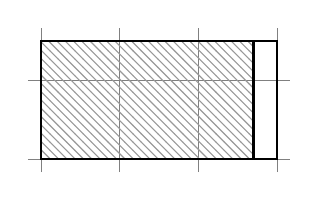
\begin{tikzpicture}[show background grid]
\pgfmathsetmacro{\laenge}{3}  
\pgfmathsetmacro{\hoehe}{\laenge/2}  
\pgfmathsetmacro{\percent}{90/100}  
\draw[thick] (0,0) rectangle ++ (\laenge,\hoehe);
\draw[thick,pattern=north west lines, pattern color=black!40] (0,0) rectangle ++ (\laenge*\percent,\hoehe);
\end{tikzpicture}
\\\hline
\end{xltabular}
\vspace{0.5cm}
\subsection{Prozentwert berechnenHS}
Füge hier bitte einen Beschreibungstext ein. Behalte die beiden Backslash \textbackslash\textbackslash. Die bedeuten eine neue Zeile. Soll die Aufgabe nicht auf einer neuen Seite beginnen, entferne den Befehl \textbackslash newpage am Anfang der tex-Datei.\\
\begin{xltabular}{\textwidth}{|C{0.75cm}|X|}
\arrayrulecolor{black}\hline
a)&Grundwert~400~Schüler;  Prozentsatz~4~\%
\\\hline
\end{xltabular}
\vspace{0.5cm}
\subsection{Kapital berechnen}
Füge hier bitte einen Beschreibungstext ein. Behalte die beiden Backslash \textbackslash\textbackslash. Die bedeuten eine neue Zeile. Soll die Aufgabe nicht auf einer neuen Seite beginnen, entferne den Befehl \textbackslash newpage am Anfang der tex-Datei.\\
\begin{xltabular}{\textwidth}{|C{0.75cm}|X|}
\arrayrulecolor{black}\hline
a)&Zinsen~174~€;  Zinssatz~5~\%
\\\hline
\end{xltabular}
\vspace{0.5cm}
\subsection{Monatszinsen einfach berechnen}
Füge hier bitte einen Beschreibungstext ein. Behalte die beiden Backslash \textbackslash\textbackslash. Die bedeuten eine neue Zeile. Soll die Aufgabe nicht auf einer neuen Seite beginnen, entferne den Befehl \textbackslash newpage am Anfang der tex-Datei.\\
\begin{xltabular}{\textwidth}{|C{0.75cm}|X|}
\arrayrulecolor{black}\hline
a)&Berechne die Monatszinsen für 5 Monate und $K=3.800~€$ bei $p~\%=5~\%$.
\\\hline
\end{xltabular}
\vspace{0.5cm}
\subsection{Grundwert berechnen HS}
Füge hier bitte einen Beschreibungstext ein. Behalte die beiden Backslash \textbackslash\textbackslash. Die bedeuten eine neue Zeile. Soll die Aufgabe nicht auf einer neuen Seite beginnen, entferne den Befehl \textbackslash newpage am Anfang der tex-Datei.\\
\begin{xltabular}{\textwidth}{|C{0.75cm}|X|}
\arrayrulecolor{black}\hline
a)&Prozentwert~1~Buntstifte;  Prozentsatz~4~\%
\\\hline
\end{xltabular}
\vspace{0.5cm}
\subsection{Zinsatz berechnen}
Füge hier bitte einen Beschreibungstext ein. Behalte die beiden Backslash \textbackslash\textbackslash. Die bedeuten eine neue Zeile. Soll die Aufgabe nicht auf einer neuen Seite beginnen, entferne den Befehl \textbackslash newpage am Anfang der tex-Datei.\\
\begin{xltabular}{\textwidth}{|C{0.75cm}|X|}
\arrayrulecolor{black}\hline
a)&Kapital~2.000~€;  Zinsen~140~€
\\\hline
\end{xltabular}
\vspace{0.5cm}
\subsection{Zinsen berechnen}
Füge hier bitte einen Beschreibungstext ein. Behalte die beiden Backslash \textbackslash\textbackslash. Die bedeuten eine neue Zeile. Soll die Aufgabe nicht auf einer neuen Seite beginnen, entferne den Befehl \textbackslash newpage am Anfang der tex-Datei.\\
\begin{xltabular}{\textwidth}{|C{0.75cm}|X|}
\arrayrulecolor{black}\hline
a)&Kapital~10.000~€;  Zinssatz~1,4~\%
\\\hline
\end{xltabular}
\vspace{0.5cm}
\subsection{Erkennen den Prozentwert im Kreis}
Füge hier bitte einen Beschreibungstext ein. Behalte die beiden Backslash \textbackslash\textbackslash. Die bedeuten eine neue Zeile. Soll die Aufgabe nicht auf einer neuen Seite beginnen, entferne den Befehl \textbackslash newpage am Anfang der tex-Datei.\\
\begin{xltabular}{\textwidth}{|C{0.75cm}|X|}
\arrayrulecolor{black}\hline
a)&\tikzstyle{background grid}=[draw, black!15,step=.5cm]
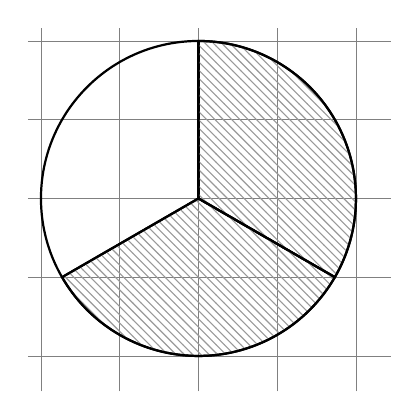
\begin{tikzpicture}[show background grid]
\pgfmathsetmacro{\R}{2}   
\draw[thick] (0,0) circle (\R); 
\draw[thick] (0,0) -- (90.0:\R);
\draw[thick] (0,0) -- (210.0:\R);
\draw[thick] (0,0) -- (330.0:\R);
\draw[thick,pattern=north west lines, pattern color=black!40] (0,0) -- (330.0:\R) arc (330.0:450.0:\R) -- (0,0);
\draw[thick,pattern=north west lines, pattern color=black!40] (0,0) -- (210.0:\R) arc (210.0:330.0:\R) -- (0,0);
\end{tikzpicture}
\\\hline
b)&\tikzstyle{background grid}=[draw, black!15,step=.5cm]
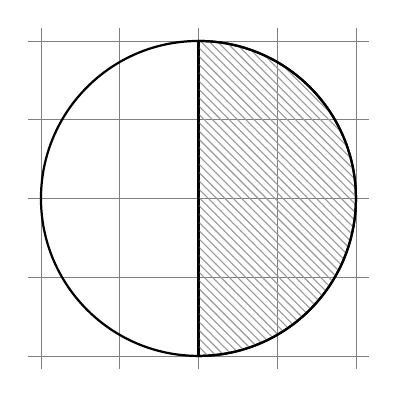
\begin{tikzpicture}[show background grid]
\pgfmathsetmacro{\R}{2}   
\draw[thick] (0,0) circle (\R); 
\draw[thick] (0,0) -- (90.0:\R);
\draw[thick] (0,0) -- (270.0:\R);
\draw[thick,pattern=north west lines, pattern color=black!40] (0,0) -- (270.0:\R) arc (270.0:450.0:\R) -- (0,0);
\end{tikzpicture}
\\\hline
\end{xltabular}
\vspace{0.5cm}
\subsection{Prozentsatz berechnen HS}
Füge hier bitte einen Beschreibungstext ein. Behalte die beiden Backslash \textbackslash\textbackslash. Die bedeuten eine neue Zeile. Soll die Aufgabe nicht auf einer neuen Seite beginnen, entferne den Befehl \textbackslash newpage am Anfang der tex-Datei.\\
\begin{xltabular}{\textwidth}{|C{0.75cm}|X|}
\arrayrulecolor{black}\hline
a)&Grundwert~500~Jungs;  Prozentwert~50~Jungs
\\\hline
\end{xltabular}
\vspace{0.5cm}
\subsection{Einfache Zinseszins Rechnung}
Füge hier bitte einen Beschreibungstext ein. Behalte die beiden Backslash \textbackslash\textbackslash. Die bedeuten eine neue Zeile. Soll die Aufgabe nicht auf einer neuen Seite beginnen, entferne den Befehl \textbackslash newpage am Anfang der tex-Datei.\\
\begin{xltabular}{\textwidth}{|C{0.75cm}|X|}
\arrayrulecolor{black}\hline
a)&Berechne das ersparte Geld nach 2 Jahren für K=7.250 € und p\%=4 \%
\\\hline
\end{xltabular}
\vspace{0.5cm}
\begin{flushright}
\underline{\hspace{2cm}/ \punkte~Punkte}
\end{flushright}
\pgfmathsetmacro{\punkte}{\pkteAfgZwei}
\newpage
\section{Textaufgaben}
\begin{enumerate}[a)]
\item Bearbeite diese Liste nach bedarf.
\item Führe dazu folgende Schritte durch.
\begin{enumerate}[1.]
\item Das item ist ein Listeneintrag
\item Ändere items zu eigenen Aufgaben
\item Füge neue items hinzu.
\item Oder entferne die, die zu viel sind.
\end{enumerate}
\item Denke auch an die korrekte Punktevergabe.
\item Brauchst du keine Textaufgabe, lösche den Inhalt dieser Datei und setze die Punkte auf 0
\item Solltest du vor den Textaufgaben keine neue Seite wünschen, entferne den Befehl \textbackslash newpage.
\end{enumerate}
\begin{flushright}
\underline{\hspace{2cm}/ \punkte~Punkte}
\end{flushright}
\end{document}